% Options for packages loaded elsewhere
% Options for packages loaded elsewhere
\PassOptionsToPackage{unicode}{hyperref}
\PassOptionsToPackage{hyphens}{url}
%
\documentclass[
  english,
  russian,
  12pt,
  a4paper,
  DIV=11,
  numbers=noendperiod]{scrreprt}
\usepackage{xcolor}
\usepackage{amsmath,amssymb}
\setcounter{secnumdepth}{5}
\usepackage{iftex}
\ifPDFTeX
  \usepackage[T1]{fontenc}
  \usepackage[utf8]{inputenc}
  \usepackage{textcomp} % provide euro and other symbols
\else % if luatex or xetex
  \usepackage{unicode-math} % this also loads fontspec
  \defaultfontfeatures{Scale=MatchLowercase}
  \defaultfontfeatures[\rmfamily]{Ligatures=TeX,Scale=1}
\fi
\usepackage{lmodern}
\ifPDFTeX\else
  % xetex/luatex font selection
\fi
% Use upquote if available, for straight quotes in verbatim environments
\IfFileExists{upquote.sty}{\usepackage{upquote}}{}
\IfFileExists{microtype.sty}{% use microtype if available
  \usepackage[]{microtype}
  \UseMicrotypeSet[protrusion]{basicmath} % disable protrusion for tt fonts
}{}
\usepackage{setspace}
% Make \paragraph and \subparagraph free-standing
\makeatletter
\ifx\paragraph\undefined\else
  \let\oldparagraph\paragraph
  \renewcommand{\paragraph}{
    \@ifstar
      \xxxParagraphStar
      \xxxParagraphNoStar
  }
  \newcommand{\xxxParagraphStar}[1]{\oldparagraph*{#1}\mbox{}}
  \newcommand{\xxxParagraphNoStar}[1]{\oldparagraph{#1}\mbox{}}
\fi
\ifx\subparagraph\undefined\else
  \let\oldsubparagraph\subparagraph
  \renewcommand{\subparagraph}{
    \@ifstar
      \xxxSubParagraphStar
      \xxxSubParagraphNoStar
  }
  \newcommand{\xxxSubParagraphStar}[1]{\oldsubparagraph*{#1}\mbox{}}
  \newcommand{\xxxSubParagraphNoStar}[1]{\oldsubparagraph{#1}\mbox{}}
\fi
\makeatother


\usepackage{longtable,booktabs,array}
\usepackage{calc} % for calculating minipage widths
% Correct order of tables after \paragraph or \subparagraph
\usepackage{etoolbox}
\makeatletter
\patchcmd\longtable{\par}{\if@noskipsec\mbox{}\fi\par}{}{}
\makeatother
% Allow footnotes in longtable head/foot
\IfFileExists{footnotehyper.sty}{\usepackage{footnotehyper}}{\usepackage{footnote}}
\makesavenoteenv{longtable}
\usepackage{graphicx}
\makeatletter
\newsavebox\pandoc@box
\newcommand*\pandocbounded[1]{% scales image to fit in text height/width
  \sbox\pandoc@box{#1}%
  \Gscale@div\@tempa{\textheight}{\dimexpr\ht\pandoc@box+\dp\pandoc@box\relax}%
  \Gscale@div\@tempb{\linewidth}{\wd\pandoc@box}%
  \ifdim\@tempb\p@<\@tempa\p@\let\@tempa\@tempb\fi% select the smaller of both
  \ifdim\@tempa\p@<\p@\scalebox{\@tempa}{\usebox\pandoc@box}%
  \else\usebox{\pandoc@box}%
  \fi%
}
% Set default figure placement to htbp
\def\fps@figure{htbp}
\makeatother



\ifLuaTeX
\usepackage[bidi=basic,provide=*]{babel}
\else
\usepackage[bidi=default,provide=*]{babel}
\fi
% get rid of language-specific shorthands (see #6817):
\let\LanguageShortHands\languageshorthands
\def\languageshorthands#1{}


\setlength{\emergencystretch}{3em} % prevent overfull lines

\providecommand{\tightlist}{%
  \setlength{\itemsep}{0pt}\setlength{\parskip}{0pt}}



 
\usepackage[style=gost-numeric,backend=biber,langhook=extras,autolang=other*]{biblatex}
\addbibresource{bib/cite.bib}

\usepackage[]{csquotes}

\KOMAoption{captions}{tableheading}
\usepackage{indentfirst}
\usepackage{float}
\floatplacement{figure}{H}
\usepackage{libertine}
\usepackage{indentfirst}
\usepackage{float}
\floatplacement{figure}{H}
\usepackage[math,RM={Scale=0.94},SS={Scale=0.94},SScon={Scale=0.94},TT={Scale=MatchLowercase,FakeStretch=0.9},DefaultFeatures={Ligatures=Common}]{plex-otf}
\makeatletter
\@ifpackageloaded{caption}{}{\usepackage{caption}}
\AtBeginDocument{%
\ifdefined\contentsname
  \renewcommand*\contentsname{Содержание}
\else
  \newcommand\contentsname{Содержание}
\fi
\ifdefined\listfigurename
  \renewcommand*\listfigurename{Список иллюстраций}
\else
  \newcommand\listfigurename{Список иллюстраций}
\fi
\ifdefined\listtablename
  \renewcommand*\listtablename{Список таблиц}
\else
  \newcommand\listtablename{Список таблиц}
\fi
\ifdefined\figurename
  \renewcommand*\figurename{Рисунок}
\else
  \newcommand\figurename{Рисунок}
\fi
\ifdefined\tablename
  \renewcommand*\tablename{Таблица}
\else
  \newcommand\tablename{Таблица}
\fi
}
\@ifpackageloaded{float}{}{\usepackage{float}}
\floatstyle{ruled}
\@ifundefined{c@chapter}{\newfloat{codelisting}{h}{lop}}{\newfloat{codelisting}{h}{lop}[chapter]}
\floatname{codelisting}{Список}
\newcommand*\listoflistings{\listof{codelisting}{Листинги}}
\makeatother
\makeatletter
\makeatother
\makeatletter
\@ifpackageloaded{caption}{}{\usepackage{caption}}
\@ifpackageloaded{subcaption}{}{\usepackage{subcaption}}
\makeatother
\usepackage{bookmark}
\IfFileExists{xurl.sty}{\usepackage{xurl}}{} % add URL line breaks if available
\urlstyle{same}
\hypersetup{
  pdftitle={Лабораторная работа №7},
  pdfauthor={Перфилов Александр Константинович \textbar{} группа НПИбд 03-24},
  pdflang={ru-RU},
  hidelinks,
  pdfcreator={LaTeX via pandoc}}


\title{Лабораторная работа №7}
\usepackage{etoolbox}
\makeatletter
\providecommand{\subtitle}[1]{% add subtitle to \maketitle
  \apptocmd{\@title}{\par {\large #1 \par}}{}{}
}
\makeatother
\subtitle{Упарвление журналами событий в системе}
\author{Перфилов Александр Константинович \textbar{} группа НПИбд 03-24}
\date{}
\begin{document}
\maketitle

\renewcommand*\contentsname{Содержание}
{
\setcounter{tocdepth}{1}
\tableofcontents
}
\listoffigures
\listoftables

\setstretch{1.5}
\chapter{Цель
работы}\label{ux446ux435ux43bux44c-ux440ux430ux431ux43eux442ux44b}

Целью данной работы является получение навыков работы с журналами
мониторинга различных событий в системе.

\chapter{Задание}\label{ux437ux430ux434ux430ux43dux438ux435}

\begin{enumerate}
\def\labelenumi{\arabic{enumi}.}
\tightlist
\item
  Продемонстрируйте навыки работы с журналом мониторинга событий в
  реальном времени (см. раздел 7.4.1).
\item
  Продемонстрируйте навыки создания и настройки отдельного файла
  конфигурации мониторинга отслеживания событий веб-службы (см. раздел
  7.4.2).
\item
  Продемонстрируйте навыки работы с journalctl (см. раздел 7.4.3).
\item
  Продемонстрируйте навыки работы с journald (см. раздел 7.4.4).
\end{enumerate}

\chapter{Выполнение лабораторной
работы}\label{ux432ux44bux43fux43eux43bux43dux435ux43dux438ux435-ux43bux430ux431ux43eux440ux430ux442ux43eux440ux43dux43eux439-ux440ux430ux431ux43eux442ux44b}

\section{Мониторинг журнала системных событий в реальном
времени}\label{ux43cux43eux43dux438ux442ux43eux440ux438ux43dux433-ux436ux443ux440ux43dux430ux43bux430-ux441ux438ux441ux442ux435ux43cux43dux44bux445-ux441ux43eux431ux44bux442ux438ux439-ux432-ux440ux435ux430ux43bux44cux43dux43eux43c-ux432ux440ux435ux43cux435ux43dux438}

Для начала запустим три вкладки терминала и в каждом из них получим
полномочия администратора: su -. На второй вкладке терминала запустим
мониторинг системных событий в реальном времени: tail -f
/var/log/messages (рис. \autocite*{fig:001}).

\begin{figure}

{\centering 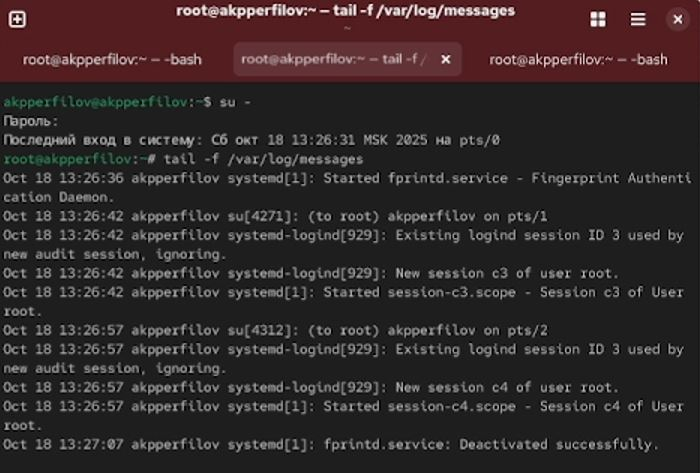
\includegraphics[width=0.71\linewidth,height=\textheight,keepaspectratio]{image/1(1).jpg}

}

\caption{Запуск трёх вкладок терминала, получение полномочий
администратора в каждой вкладке, запуск на второй вкладке терминала
мониторинга системных событий в реальном времени.}

\end{figure}%

В третьей вкладке терминала вернёмся к учётной записи своего
пользователя (нажав Ctrl + d) и попробуем получить полномочия
администратора, но при этом вводим неправильный пароль (рис.
\autocite*{fig:002}).

\begin{figure}

{\centering 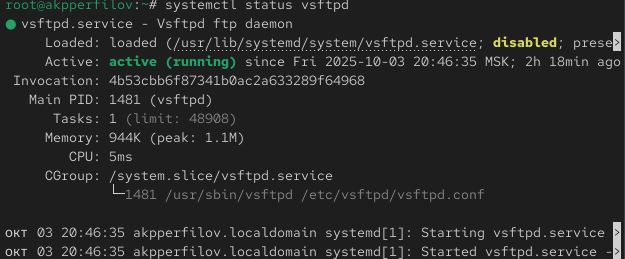
\includegraphics[width=0.7\linewidth,height=\textheight,keepaspectratio]{image/2.jpg}

}

\caption{Возвращение учётной записи своего пользователя в третьей
вкладке терминала, попытка получения полномочий администратора.}

\end{figure}%

Обратим внимание, что во второй вкладке терминала с мониторингом событий
появилось сообщение «FAILED SU (to root) mobihzova on pts/2».
Отображаемые на экране сообщения также фиксируются в файле
/var/log/messages (рис. \autocite*{fig:003}).

\begin{figure}

{\centering 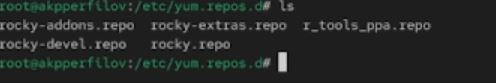
\includegraphics[width=0.7\linewidth,height=\textheight,keepaspectratio]{image/3.jpg}

}

\caption{Новое сообщение в мониторинге событий во второй вкладке
терминала.}

\end{figure}%

В третьей вкладке терминала из оболочки пользователя введём: logger
hello (рис. \autocite*{fig:004}).

\begin{figure}

{\centering 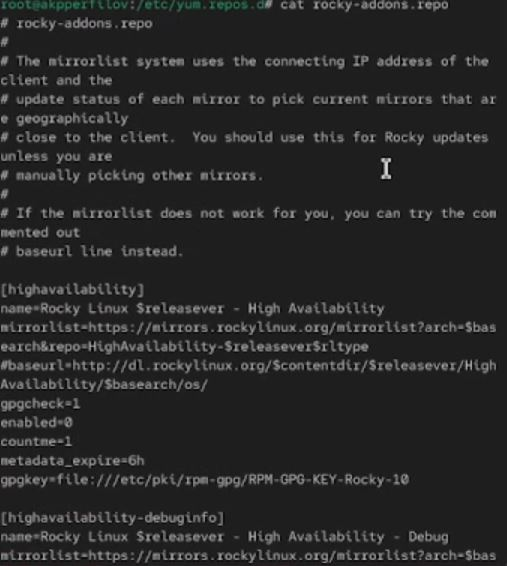
\includegraphics[width=0.7\linewidth,height=\textheight,keepaspectratio]{image/4.jpg}

}

\caption{Ввод в третьей вкладке терминала.}

\end{figure}%

Далее возвращаемся во вторую вкладку терминала с мониторингом событий и
видим сообщение, которое также будет зафиксировано в файле
/var/log/messages («hello»). В этой же вкладке терминала с мониторингом
остановим трассировку файла сообщений мониторинга реального времени,
используя Ctrl + c.~Затем запустим мониторинг сообщений безопасности
(последние 20 строк соответствующего файла логов): tail -n 20
/var/log/secure. Мы видим сообщения, которые ранее были зафиксированы во
время ошибки авторизации при вводе команды su - (рис.
\autocite*{fig:005}).

\begin{figure}

{\centering 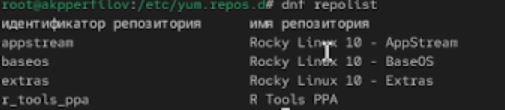
\includegraphics[width=0.7\linewidth,height=\textheight,keepaspectratio]{image/5.jpg}

}

\caption{Возвращение во вторую вкладку терминала с мониторингом событий,
просмотр сообщения, остановка трассировки файла сообщений мониторинга
реального времени, запуск мониторинга сообщений безопасности (последние
20 строк).}

\end{figure}%

\section{Изменение правил
rsyslog.conf}\label{ux438ux437ux43cux435ux43dux435ux43dux438ux435-ux43fux440ux430ux432ux438ux43b-rsyslog.conf}

В первой вкладке терминала установим Apache: dnf -y install httpd (рис.
\autocite*{fig:006}).

\begin{figure}

{\centering 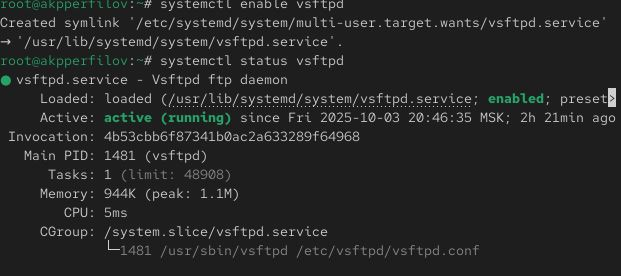
\includegraphics[width=0.7\linewidth,height=\textheight,keepaspectratio]{image/6.jpg}

}

\caption{Установка Apache.}

\end{figure}%

После окончания процесса установки запустим веб-службу: systemctl start
httpd и systemctl enable httpd (рис. \autocite*{fig:007}).

\begin{figure}

{\centering 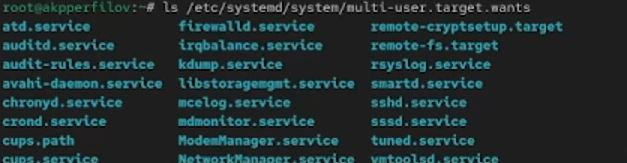
\includegraphics[width=0.7\linewidth,height=\textheight,keepaspectratio]{image/7.jpg}

}

\caption{Запуск веб-службы.}

\end{figure}%

Во второй вкладке терминала посмотрим журнал сообщений об ошибках веб-
службы: tail -f /var/log/httpd/error\_log. Чтобы закрыть трассировку
файла журнала, используем Ctrl + c (рис. \autocite*{fig:008}).

\begin{figure}

{\centering 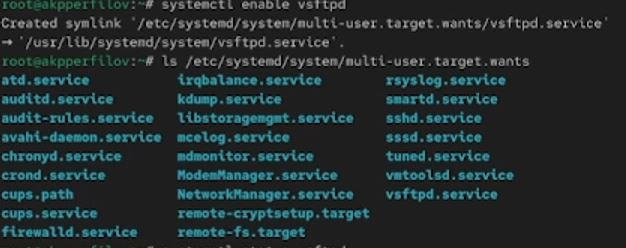
\includegraphics[width=0.7\linewidth,height=\textheight,keepaspectratio]{image/8.jpg}

}

\caption{Просмотр журнала сообщений об ошибках веб-службы, закрытие
трассировки файла журнала.}

\end{figure}%

В третьей вкладке терминала получим полномочия администратора и в файле
конфигурации /etc/httpd/conf/httpd.conf в конце добавляем следующую
строку: ErrorLog syslog:local (рис. \autocite*{fig:009}, рис.
\autocite*{fig:010}).

Здесь local0 --- local7 --- это «настраиваемые» средства (объекты),
которые syslog предоставляет пользователю для регистрации событий
приложения в системном журнале.

\begin{figure}

{\centering 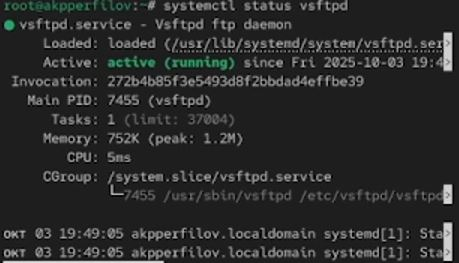
\includegraphics[width=0.7\linewidth,height=\textheight,keepaspectratio]{image/9.jpg}

}

\caption{Получение в третьей вкладке терминала полномочия
администратора, открытие файла httpd.conf на редактирование.}

\end{figure}%

\begin{figure}

{\centering 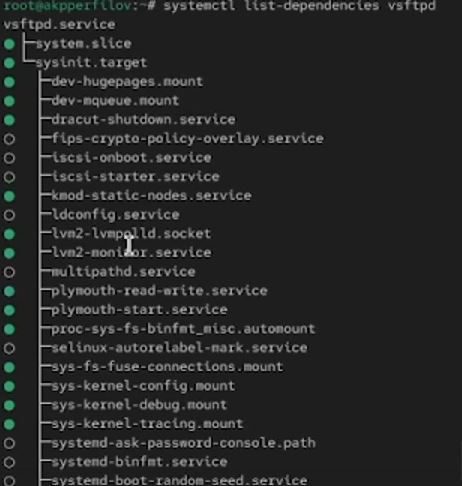
\includegraphics[width=0.7\linewidth,height=\textheight,keepaspectratio]{image/10.jpg}

}

\caption{Добавление строки в файл и сохранение.}

\end{figure}%

В каталоге /etc/rsyslog.d создаём файл мониторинга событий веб-службы:

cd /etc/rsyslog.d touch httpd.conf

Открыв его на редактирование, пропишем в нём local1.*
-/var/log/httpd-error.log (Рис. 2.7). Эта строка позволит отправлять все
сообщения, получаемые для объекта local1 (который теперь используется
службой httpd), в файл /var/log/httpderror.log (рис.
\autocite*{fig:011}, рис. \autocite*{fig:012}).

\begin{figure}

{\centering 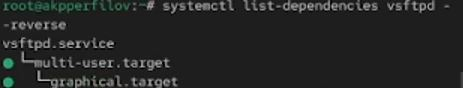
\includegraphics[width=0.7\linewidth,height=\textheight,keepaspectratio]{image/11.jpg}

}

\caption{Создание в каталоге /etc/rsyslog.d файла мониторинга событий
веб-службы и открытие его на редактирование.}

\end{figure}%

\begin{figure}

{\centering 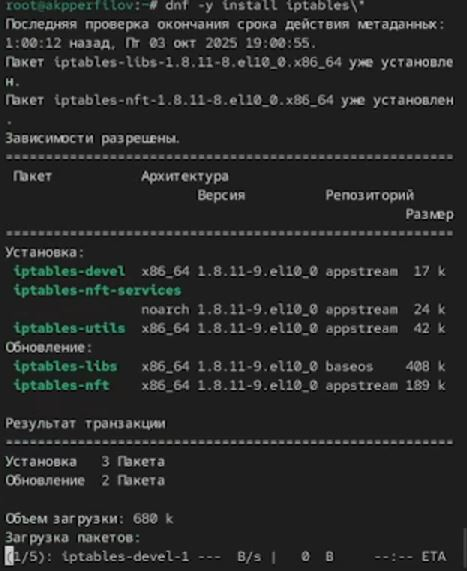
\includegraphics[width=0.7\linewidth,height=\textheight,keepaspectratio]{image/12.jpg}

}

\caption{Добавление строки в файл и сохранение.}

\end{figure}%

Перейдём в первую вкладку терминала и перезагрузим конфигурацию rsyslogd
и веб-службу:

systemctl restart rsyslog.service systemctl restart httpd

Все сообщения об ошибках веб-службы теперь будут записаны в файл
/var/log/httpd-error.log, что можно наблюдать или в режиме реального
времени, используя команду tail с соответствующими параметрами, или
непосредственно просматривая указанный файл. (рис. \autocite*{fig:013}).

\begin{figure}

{\centering 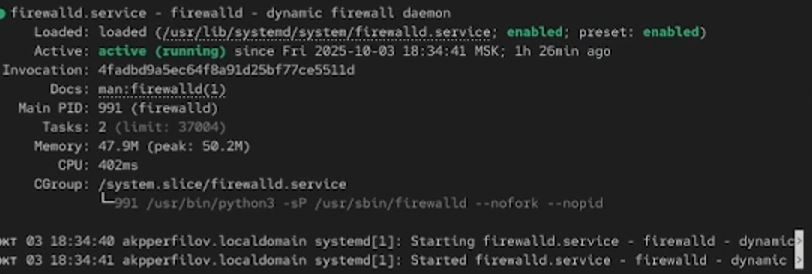
\includegraphics[width=0.7\linewidth,height=\textheight,keepaspectratio]{image/13.jpg}

}

\caption{Открытие первой вкладки терминала и перезагрузка конфигурации
rsyslogd и веб-службы.}

\end{figure}%

В третьей вкладке терминала создаём отдельный файл конфигурации для
мониторинга отладочной информации:

cd /etc/rsyslog.d touch debug.conf

В этом же терминале вводим: echo ``*.debug /var/log/messages-debug''
\textgreater{} /etc/rsyslog.d/debug.conf (рис. \autocite*{fig:014}).

\begin{figure}

{\centering 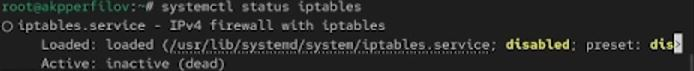
\includegraphics[width=0.7\linewidth,height=\textheight,keepaspectratio]{image/14.jpg}

}

\caption{Открытие третьей вкладки терминала, создание отдельного файла
конфигурации для мониторинга отладочной информации, ввод заданной
строки.}

\end{figure}%

В первой вкладке терминала снова перезапустим rsyslogd: systemctl
restart rsyslog.service (рис. \autocite*{fig:015}).

\begin{figure}

{\centering 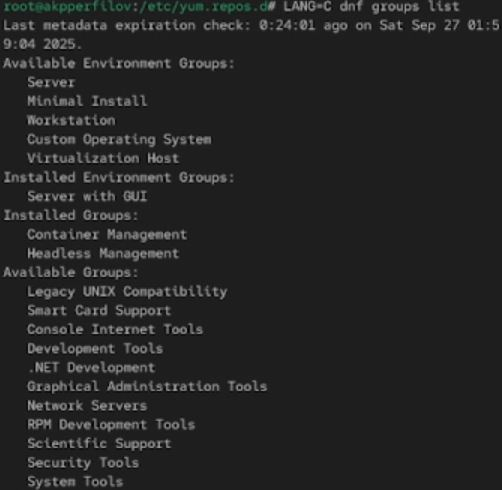
\includegraphics[width=0.7\linewidth,height=\textheight,keepaspectratio]{image/15.jpg}

}

\caption{Открытие первой вкладки терминала и перезапуск rsyslogd.}

\end{figure}%

Во второй вкладке терминала запустим мониторинг отладочной информации:
tail -f /var/log/messages-debug (рис. \autocite*{fig:016}).

\begin{figure}

{\centering 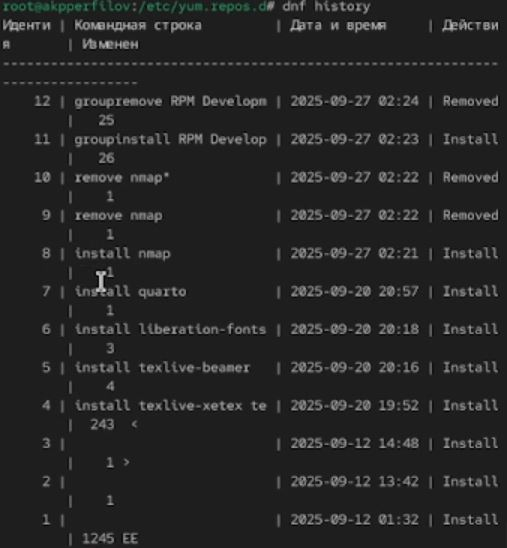
\includegraphics[width=0.7\linewidth,height=\textheight,keepaspectratio]{image/16.jpg}

}

\caption{Открытие второй вкладки терминала и запуск мониторинга
отладочной информации.}

\end{figure}%

В третьей вкладке терминала введём: logger -p daemon.debug
\enquote{Daemon Debug Message} (рис. \autocite*{fig:017}).

\begin{figure}

{\centering 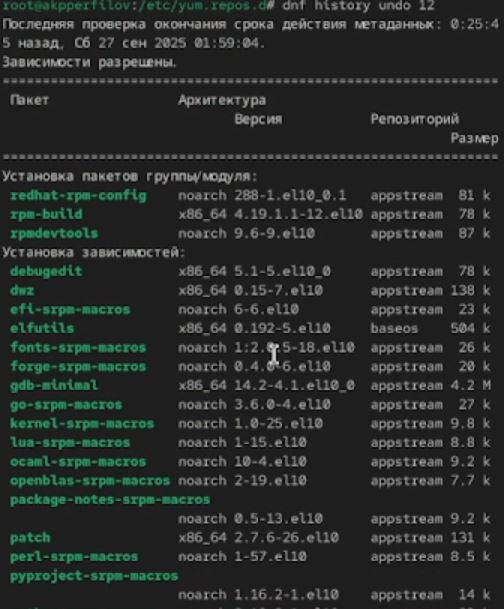
\includegraphics[width=0.7\linewidth,height=\textheight,keepaspectratio]{image/17.jpg}

}

\caption{Открытие третьей вкладки терминала и ввод команды.}

\end{figure}%

В терминале с мониторингом посмотрим сообщение отладки. Чтобы закрыть
трассировку файла журнала, используем Ctrl + c (рис.
\autocite*{fig:018}).

\begin{figure}

{\centering 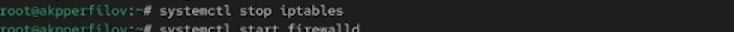
\includegraphics[width=0.7\linewidth,height=\textheight,keepaspectratio]{image/18.jpg}

}

\caption{Просмотр сообщения отладки и закрытие трассировки файла
журнала.}

\end{figure}%

\section{Использование
journalctl}\label{ux438ux441ux43fux43eux43bux44cux437ux43eux432ux430ux43dux438ux435-journalctl}

Во второй вкладке терминала посмотрим содержимое журнала с событиями с
момента последнего запуска системы: journalctl. Для пролистывания
журнала можно использовать или Enter (построчный просмотр), или пробел
(постраничный просмотр). Для выхода из просмотра используется q (рис.
\autocite*{fig:019}).

\begin{figure}

{\centering 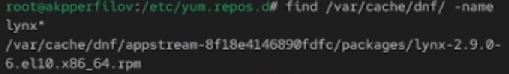
\includegraphics[width=0.7\linewidth,height=\textheight,keepaspectratio]{image/19.jpg}

}

\caption{Открытие второй вкладки терминала и просмотр содержимого
журнала с событиями с момента последнего запуска системы.}

\end{figure}%

Просмотрим содержимое журнала без использования пейджера: journalctl --
no-pager (рис. \autocite*{fig:020}).

\begin{figure}

{\centering 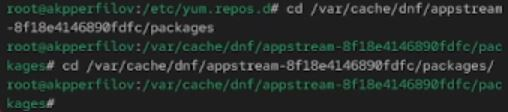
\includegraphics[width=0.7\linewidth,height=\textheight,keepaspectratio]{image/20.jpg}

}

\caption{Просмотр содержимого журнала без использования пейджера.}

\end{figure}%

Режим просмотра журнала в реальном времени: journalctl -f.~Для
прерывания просмотра: Ctrl + c (рис. \autocite*{fig:021}).

\begin{figure}

{\centering 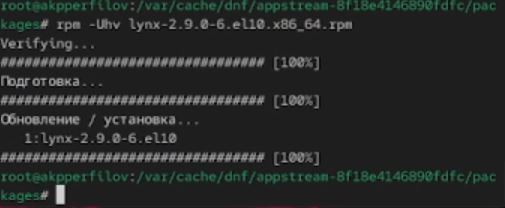
\includegraphics[width=0.7\linewidth,height=\textheight,keepaspectratio]{image/21.jpg}

}

\caption{Режим просмотра журнала в реальном времени и прерывание
просмотра.}

\end{figure}%

Просмотрим события для UID0: journalctl \_UID=0 (рис.
\autocite*{fig:022}).

\begin{figure}

{\centering 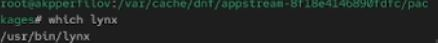
\includegraphics[width=0.7\linewidth,height=\textheight,keepaspectratio]{image/22.jpg}

}

\caption{Просмотр событий для UID0.}

\end{figure}%

Для отображения последних 20 строк журнала введём: journalctl -n 20
(рис. \autocite*{fig:023}).

\begin{figure}

{\centering 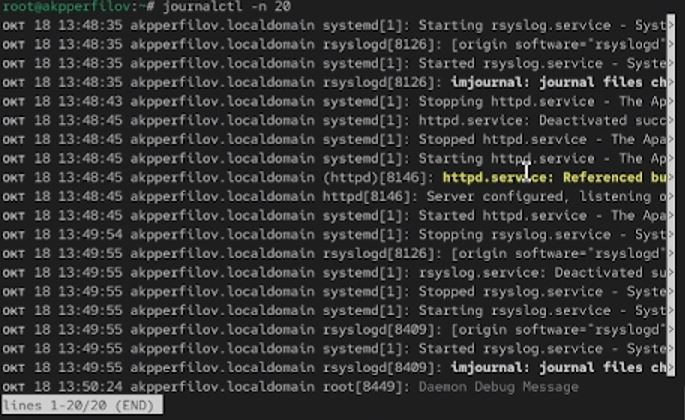
\includegraphics[width=0.7\linewidth,height=\textheight,keepaspectratio]{image/23(1).jpg}

}

\caption{Отображение последних 20 строк журнала.}

\end{figure}%

Для просмотра только сообщений об ошибках введём: journalctl -p err
(рис. \autocite*{fig:024}).

\begin{figure}

{\centering 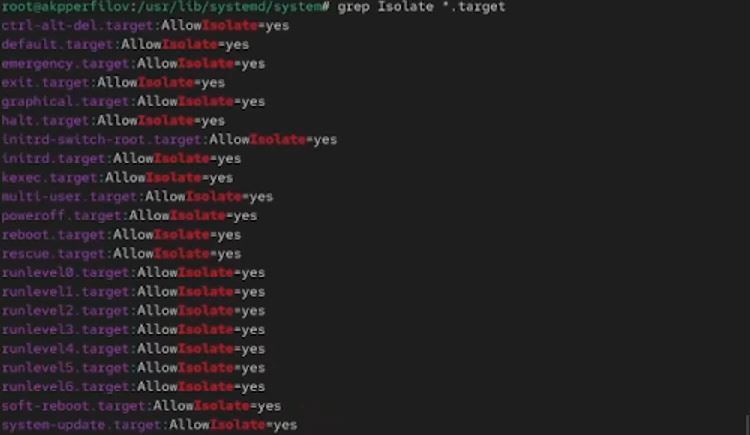
\includegraphics[width=0.7\linewidth,height=\textheight,keepaspectratio]{image/24.jpg}

}

\caption{Просмотр только сообщений об ошибках.}

\end{figure}%

Если мы хотим просмотреть сообщения журнала, записанные за определённый
период времени, мы можем использовать параметры --since и -- until. Обе
опции принимают параметр времени в формате YYYY-MM-DD hh:mm:ss Кроме
того, мы можем использовать yesterday, today и tomorrow в качестве
параметров. Например, для просмотра всех сообщений со вчерашнего дня
введём: journalctl --since yesterday (рис. \autocite*{fig:025}).

\begin{figure}

{\centering 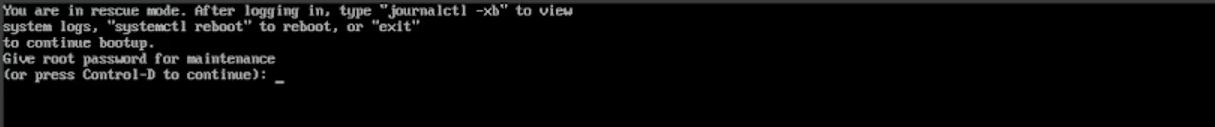
\includegraphics[width=0.7\linewidth,height=\textheight,keepaspectratio]{image/25.jpg}

}

\caption{Просмотр всех сообщений со вчерашнего дня.}

\end{figure}%

Если мы хотим показать все сообщения с ошибкой приоритета, которые были
зафиксированы со вчерашнего дня, то используем: journalctl --since
yesterday - p err, а если нам нужна детальная информация, то используем:
journalctl -o verbose (рис. \autocite*{fig:026}).

\begin{figure}

{\centering 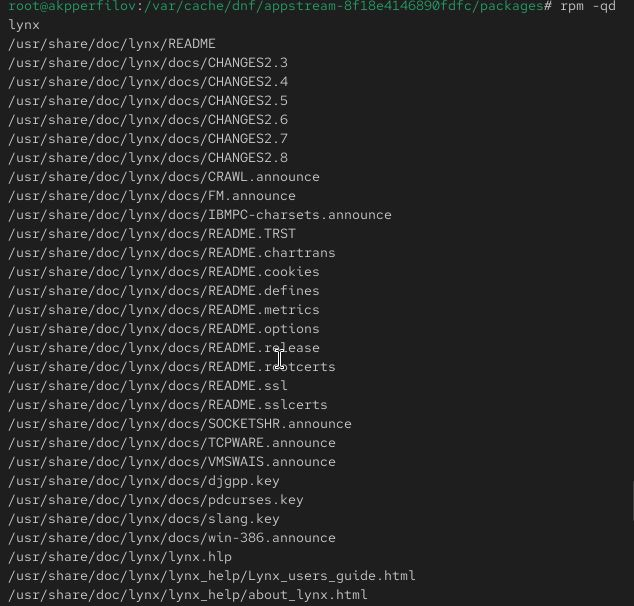
\includegraphics[width=0.7\linewidth,height=\textheight,keepaspectratio]{image/26.jpg}

}

\caption{Просмотр сообщений с ошибкой приоритета, которые были
зафиксированы со вчерашнего дня. Просмотр детальной информации.}

\end{figure}%

Для просмотра дополнительной информации о модуле sshd введём: journalctl
\_SYSTEMD\_UNIT=sshd.service (рис. \autocite*{fig:027}).

\begin{figure}

{\centering 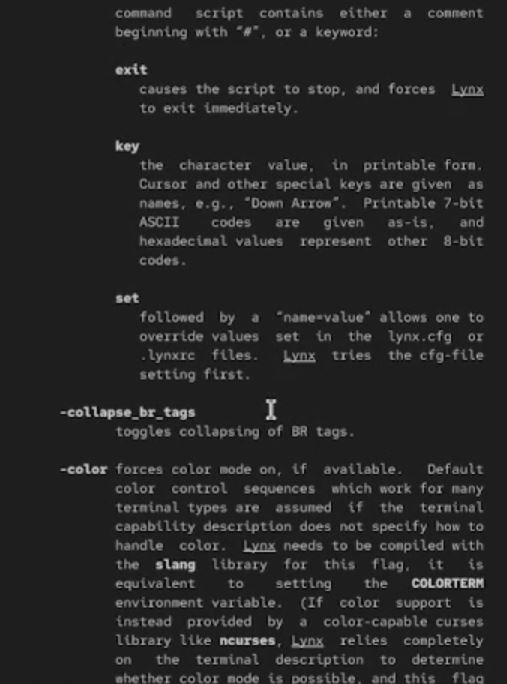
\includegraphics[width=0.7\linewidth,height=\textheight,keepaspectratio]{image/27.jpg}

}

\caption{Просмотр дополнительной информации о модуле sshd.}

\end{figure}%

\section{Постоянный журнал
journald}\label{ux43fux43eux441ux442ux43eux44fux43dux43dux44bux439-ux436ux443ux440ux43dux430ux43b-journald}

Запустим терминал и получим полномочия администратора: su -. Далее
создадим каталог для хранения записей журнала: mkdir -p /var/log/journal
и скорректируем права доступа для каталога /var/log/journal, чтобы
journald смог записывать в него информацию:

chown root:systemd-journal /var/log/journal chmod 2755 /var/log/journal

Для принятия изменений необходимо использовать команду: killall -USR1
systemd-journald. Журнал systemd теперь постоянный. Если мы хотим видеть
сообщения журнала с момента последней перезагрузки, используем:
journalctl -b (рис. \autocite*{fig:028}).

\begin{figure}

{\centering 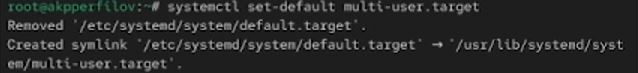
\includegraphics[width=0.7\linewidth,height=\textheight,keepaspectratio]{image/28.jpg}

}

\caption{Запуск терминала и получение полномочий администратора,
создание каталог для хранения записей журнала, корректировка прав
доступа для каталога /var/log/journal, принятия изменений, просмотр
сообщения журнала с момента последней перезагрузки.}

\end{figure}%

\section{Ответы на контрольные
вопросы}\label{ux43eux442ux432ux435ux442ux44b-ux43dux430-ux43aux43eux43dux442ux440ux43eux43bux44cux43dux44bux435-ux432ux43eux43fux440ux43eux441ux44b}

\begin{enumerate}
\def\labelenumi{\arabic{enumi}.}
\tightlist
\item
  Какой файл используется для настройки rsyslogd? /etc/rsyslog.conf
\end{enumerate}

\includegraphics[width=0.7\linewidth,height=\textheight,keepaspectratio]{.pdf}

\begin{enumerate}
\def\labelenumi{\arabic{enumi}.}
\setcounter{enumi}{1}
\tightlist
\item
  В каком файле журнала rsyslogd содержатся сообщения, связанные с
  аутентификацией? /var/log/secure
\end{enumerate}

\includegraphics[width=0.7\linewidth,height=\textheight,keepaspectratio]{.pdf}

\begin{enumerate}
\def\labelenumi{\arabic{enumi}.}
\setcounter{enumi}{2}
\tightlist
\item
  Если вы ничего не настроите, то сколько времени потребуется для
  ротации файлов журналов? Неделя
\end{enumerate}

\includegraphics[width=0.7\linewidth,height=\textheight,keepaspectratio]{.pdf}

\begin{enumerate}
\def\labelenumi{\arabic{enumi}.}
\setcounter{enumi}{3}
\item
  Какую строку следует добавить в конфигурацию для записи всех сообщений
  с приоритетом info в файл /var/log messages.info? info.* -
  /var/log/messages.info
\item
  Какая команда позволяет вам видеть сообщения журнала в режиме
  реального времени? tail -f /var/log/messages
\end{enumerate}

\includegraphics[width=0.7\linewidth,height=\textheight,keepaspectratio]{.pdf}

\begin{enumerate}
\def\labelenumi{\arabic{enumi}.}
\setcounter{enumi}{5}
\item
  Какая команда позволяет вам видеть все сообщения журнала, которые были
  написаны для PID 1 между 9:00 и 15:00 journalctl \_PID=1 -since
  \enquote{2022-02-01 09:00:00} --until \enquote{2022-02-01 15:00:00}
\item
  Какая команда позволяет вам видеть сообщения journald после последней
  перезагрузки системы? journalctl - b
\item
  Какая процедура позволяет сделать журнал journald постоянным?
\end{enumerate}

Запустите терминал и получите полномочия администратора: su -- Создайте
каталог для хранения записей журнала: mkdir -p /var/log/journal.
Скорректируйте права доступа для каталога /var/log/journal, чтобы
journald смог записывать в него информацию:

chown root:systemd-journal /var/log/journal chmod 2755 /var/log/journal

Для принятия изменений необходимо или перезагрузить систему
(перезапустить службу systemd-journald недостаточно), или использовать
команду: killall -USR1 systemd-journald

\includegraphics[width=0.7\linewidth,height=\textheight,keepaspectratio]{.pdf}

\chapter{Выводы}\label{ux432ux44bux432ux43eux434ux44b}

В ходе выполнения лабораторной работы были получены навыки работы с
журналами мониторинга различных событий в системе.


\printbibliography



\end{document}
